\documentclass[preprint,a4paper]{elsarticle}

\usepackage{afterpage}
\usepackage{alltt}
\usepackage{amsfonts}
\usepackage{amsmath}
\usepackage{bold-extra}
\usepackage{color}
\usepackage{float}
\usepackage{graphicx}
\usepackage{listings}
\usepackage{subfigure}
\usepackage{url}

%%%%%%%%%%%%
% Commands %
%%%%%%%%%%%%

\newcommand{\argmin}{\operatornamewithlimits{argmin}}
\newcommand{\eqdef}{\stackrel{\Delta}{=}}
\newcommand{\funcname}[1]{\mathit{#1}}

%%%%%%%%%%%%%%%
%%% Colours %%%
%%%%%%%%%%%%%%%

\definecolor{darkgreen}{rgb}{0, 0.6, 0}
\definecolor{lightgrey}{gray}{0.9}

%%%%%%%%%%%
% Figures %
%%%%%%%%%%%

% Define shorter ways to include individual images
\newcommand{\stufig}[4]						% images with default placement
{
	\begin{figure}
	\begin{center}
		\includegraphics[#1]{#2}
		\caption{#3}
		\label{#4}
	\end{center}
	\end{figure}
}

\newcommand{\stufigex}[5]					% images with specified placement
{
	\begin{figure}[#5]
	\begin{center}
		\includegraphics[#1]{#2}
		\caption{#3}
		\label{#4}
	\end{center}
	\end{figure}
}

\newcommand{\stufigexx}[5]				% full-width images with specified placement
{
	\begin{figure*}[#5]
	\begin{center}
		\includegraphics[#1]{#2}
		\caption{#3}
		\label{#4}
	\end{center}
	\end{figure*}
}

% Define the stusubfig environment
\newenvironment{stusubfig}[1]
{
	\begin{figure*}[#1]
	\begin{center}
}
{
	\end{center}
	\end{figure*}
}

%%%%%%%%%%%%%%%%%
% Code Listings %
%%%%%%%%%%%%%%%%%

% Create a new type of float (called a stulisting) for listings
\floatstyle{ruled}
\newfloat{stulisting}{thp}{lop}
\floatname{stulisting}{Listing}

% Setup before using the listings package
\renewcommand{\lstlistingname}{\textbf{Listing}}
\def\thelstlisting{\textbf{\arabic{lstlisting}}}

\lstdefinelanguage{Pseudocode}{
morekeywords={and,assert,break,case,continue,default,down,each,else,for,function,if,not,null,or,rangeswitch,ref,return,switch,then,this,throw,to,up,var,while},
sensitive=true,
morecomment=[l]{//},
morecomment=[s]{/*}{*/}
}

\lstdefinestyle{Default}{
abovecaptionskip=0.5cm,
basicstyle=\scriptsize\ttfamily,
belowcaptionskip=0.5cm,
belowskip=0.5cm,
columns=fixed,
%commentstyle=\color{darkgreen},
commentstyle=\textit, % changed from the thesis (green text looks unprofessional in a journal paper)
language=Pseudocode,
%numbers=left,
numbers=none, % changed from the thesis (line numbers are less relevant here)
numbersep=5pt,
numberstyle=\tiny,
mathescape=true,
showstringspaces=false,
stepnumber=1,
tabsize=4
}

\lstdefinestyle{Snippet}{
abovecaptionskip=0.5cm,
aboveskip=0.5cm,
basicstyle=\small\ttfamily,
belowcaptionskip=0.5cm,
belowskip=0.5cm,
columns=fixed,
commentstyle=\color{darkgreen},
frame=lines,
keywordstyle=\small\bfseries,
language=Pseudocode,
numbers=none,
mathescape=true,
showstringspaces=false,
stepnumber=1,
tabsize=4
}

% For C++ function prototypes
\lstdefinestyle{Prototype}{
abovecaptionskip=0.5cm,
basicstyle=\small\ttfamily,
belowcaptionskip=0.5cm,
belowskip=0.5cm,
columns=fixed,
commentstyle=\color{darkgreen},
language=C++,
numbers=none,
mathescape=true,
showstringspaces=false,
stepnumber=1,
tabsize=4
}

%%%%%%%%%%%%%%%%%
% Main Document %
%%%%%%%%%%%%%%%%%

\journal{Pattern Recognition}

\begin{document}

\begin{frontmatter}

\title{Two Tree-Based Methods for the Waterfall}

\author[ox]{S.M.~Golodetz\corref{cor1}\fnref{fn1}}
\ead{sgolodetz@gxstudios.net}

\author[ox]{C.~Nicholls\fnref{fn2}}
\ead{ChrisNicholls1@gmail.com}

\author[ox]{I.D.~Voiculescu\corref{cor2}}
\ead{irina@cs.ox.ac.uk}

\author[ox]{S.A.~Cameron}
\ead{cameron@cs.ox.ac.uk}

\cortext[cor1]{Principal corresponding author}
\cortext[cor2]{Corresponding author}
\fntext[fn1]{S.M.~Golodetz is now with the Nuffield Department of Clinical Neurosciences.}
\fntext[fn2]{C.~Nicholls is now with Improbable Worlds Ltd.}

\address[ox]{Department of Computer Science, University of Oxford, Wolfson Building, Parks Road, Oxford, OX1 3QD, United Kingdom}
%\address[cox]{c/o Department of Computer Science, University of Oxford, Parks Road, Oxford OX1 3QD}
%\address[iw]{Improbable Worlds, 10 Norwich Street, London EC4A 1BD}

\begin{abstract}
The waterfall transform is a hierarchical segmentation technique based on the watershed transform from the field of mathematical morphology. Watershed-based techniques are useful in numerous fields ranging from image segmentation to cell-and-portal generation for games. The waterfall helps mitigate the problem of over-segmentation that commonly occurs when applying the basic watershed transform. It can also be used as a core part of a method for constructing \emph{image partition forests}, a tree-based, multi-scale representation of an image. The best existing method for the waterfall is fast and effective, but our experience has been that it is not as straightforward to implement as might be desired. Furthermore, it does not deal consistently with the issue of non-minimal plateaux. This paper therefore proposes two new tree-based methods for the waterfall. Both are easier to implement than the existing state-of-the-art, and in our implementations were both faster by a constant factor. The Simplified Waterfall (SW) method focuses on simplicity and ease of implementation; the Balanced Waterfall (BW) method focuses on robust handling of non-minimal plateaux. We perform experiments on both 2D and 3D images to contrast the new methods with each other and with the existing state-of-the-art, and show that both achieve a noticeable speed-up whilst producing similar results.
\end{abstract}

\begin{keyword}
image segmentation \sep waterfall transform
\end{keyword}

\end{frontmatter}

%#####################
\section{Introduction}
%#####################

The waterfall transform is a hierarchical segmentation technique based on the well-known watershed transform \cite{beucher90,gonzalez02}. Given an entity (most commonly, an image), it produces a stack of nested partitions of the entity at different scales (see Figure~\ref{fig:ipfs-ctconcept}). It was originally introduced by Beucher \cite{beucher94} as a way of improving upon the often over-segmented output of the watershed (see \S\ref{sec:background}). Watershed-based techniques see use in numerous fields, including image segmentation \cite{adiga01,beucher91,desmet10,grau04,gvccimi08,peter08,klava09,tarabalka10}, 3D mesh segmentation \cite{chen06,mangan99,moumoun10a}, automatic navigation mesh generation \cite{mononen09}, cell-and-portal generation \cite{haumont03} and roadmap generation \cite{hamlin08}. It is also possible (e.g.~see \cite{golodetz11}) to make use of the watershed and waterfall transforms to construct \emph{image partition forests} (IPFs), a tree-based representation of an image created by treating each partition as an adjacency graph (with image regions as nodes) and adding parent/child links between nodes in consecutive partitions. This representation is useful for feature identification in that it provides a helpful space in which to search for image features of different sizes.

There are various existing ways of implementing the waterfall. The initial paper by Beucher \cite{beucher94} presented three methods: a slightly intricate graph-based method that works on the gradient of the mosaic image, a method based on checking for symmetric waterfalls, and a more efficient reconstruction method that works by filling in catchment basins. A fast waterfall method was presented by Marcotegui in \cite{marcotegui05}: this returns to the idea of a graph-based waterfall (using a different graph) and works on a minimum spanning tree (MST) of the graph for improved efficiency. Marcotegui's waterfall method is fast and effective, but it is somewhat fiddly to implement \cite{golodetz08} and its handling of non-minimal plateaux in the MST is not well-specified and depends on precisely how the method is implemented.

%---
\stufigex{height=10cm}{ipfs-ctconcept.png}{A stack of nested partitions produced by the watershed and waterfall for an example image. The input image (a slice from a CT scan of the abdomen) is the lowest image in the stack. It was subjected to a gradient magnitude filter and smoothed using anisotropic diffusion filtering \cite{perona90} before performing the watershed.}{fig:ipfs-ctconcept}{!t}
%---

%\pagebreak

This paper therefore presents two new tree-based methods for the waterfall. The Simplified Waterfall (SW) method is especially simple to implement and performs well, even though it does not deal consistently with non-minimal plateaux. The Balanced Waterfall (BW) method is somewhat harder to implement (although still easier to implement than Marcotegui's method) but deals consistently with non-minimal plateaux. We perform experiments to contrast the results of these methods with those of Marcotegui's approach, and time them to compare their performance.

This paper is organised as follows: in \S\ref{sec:background}, we briefly review the watershed and waterfall transforms and take a detailed look at Marcotegui's approach to the waterfall; in \S\ref{sec:nicholls} and \S\ref{sec:golodetz}, we present our new waterfall methods; in \S\ref{sec:experiments}, we perform experiments on both 2D and 3D images to contrast our new methods with Marcotegui's approach; and in \S\ref{sec:discussion}, we discuss the results of our experiments.

%#####################
\section{Background}
\label{sec:background}
%#####################

\subsection{The Watershed Transform}

At a very abstract level, the watershed transform involves dividing a landscape into its catchment basins, where a catchment basin is an area of the landscape from which water runs down to the same point (namely one of the landscape's local minima). A watershed is a boundary between adjacent catchment basins. In each domain in which the watershed transform is used, a conceptual mapping needs to be made to allow the entity being segmented to be viewed as a landscape: for example, 2D greyscale images can be viewed as a height map, where the grey value of the image at coordinates $(x,y)$ gives the height of the `landscape' at that point. In order to produce meaningful segmentations, the watershed is often performed on the gradient magnitude of an input landscape, on the basis that in many domains, features of interest can be expected to have similar heights throughout their extent. Methods that implement the watershed transform fall into two categories:

\begin{enumerate}

\item Rainfalling methods \cite{meijster98,osma-ruiz06,stoev00} work by finding a path of steepest descent from each point in the landscape and following it until a local minimum is found (see Figure~\ref{fig:segmentation-watershed-rainfallingconcept}). Most of the difficulty involved in this approach is associated with how to handle non-minimal plateaux in the landscape (flat areas that are not the base of a catchment basin).

\item Flooding (or immersion) methods \cite{bieniek00,rambabu07} simulate a process of flooding from all the local minima simultaneously and conceptually add watersheds where the pools of water from adjacent catchment basins meet. The flooding process can be visualised as taking the landscape surface, poking holes through its local minima and lowering it perpendicularly into a body of water (see Figure~\ref{fig:segmentation-watershed-floodingconcept}).

\end{enumerate}

%---
\begin{stusubfig}{p}
	\subfigure[]
	{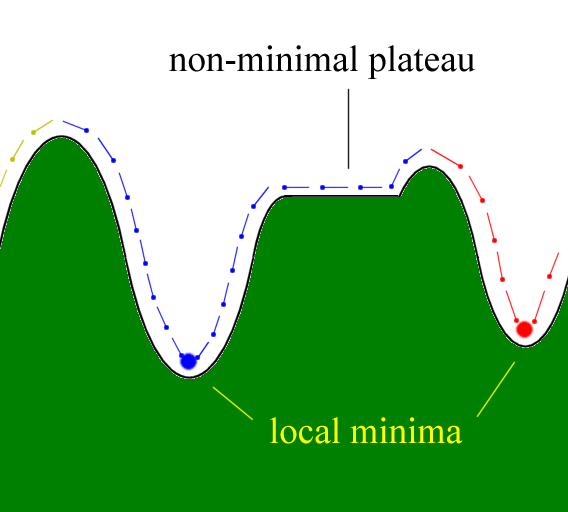
\includegraphics[height=3.5cm]{segmentation-watershed-rainfallingconcept-a.png}}%
	%
	\hspace{4mm}%
	%
	\subfigure[]
	{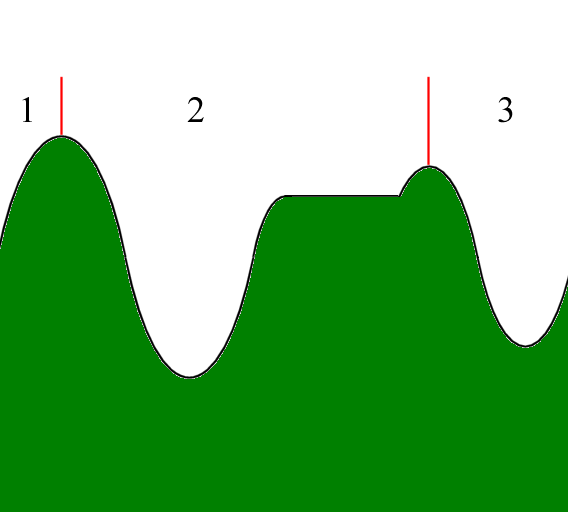
\includegraphics[height=3.5cm]{segmentation-watershed-rainfallingconcept-b.png}}%
\caption{The rainfalling concept of the watershed transform: (a) finding a path of steepest descent from each point; (b) the division of the landscape into catchment basins.}
\label{fig:segmentation-watershed-rainfallingconcept}
\end{stusubfig}
%---

%---
\begin{stusubfig}{p}
	\subfigure[]
	{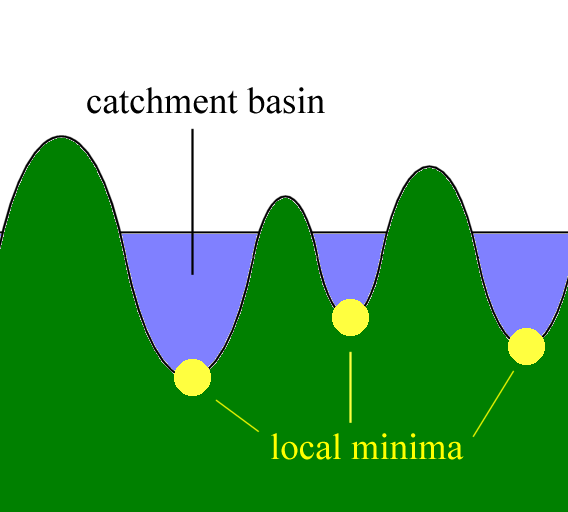
\includegraphics[width=.22\linewidth]{segmentation-watershed-floodingconcept-a.png}}%
	%
	\hspace{4mm}%
	%
	\subfigure[]
	{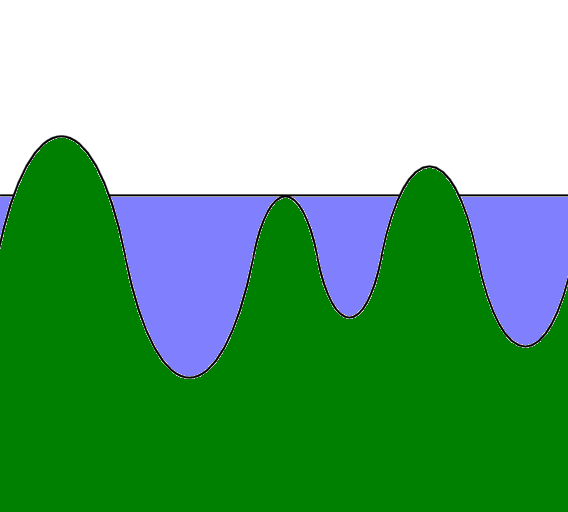
\includegraphics[width=.22\linewidth]{segmentation-watershed-floodingconcept-b.png}}%
	%
	\hspace{4mm}%
	%
	\subfigure[]
	{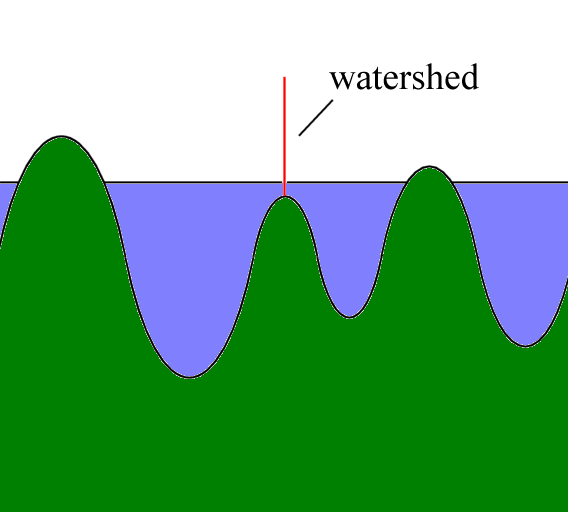
\includegraphics[width=.22\linewidth]{segmentation-watershed-floodingconcept-c.png}}%
	%
	\hspace{4mm}%
	%
	\subfigure[]
	{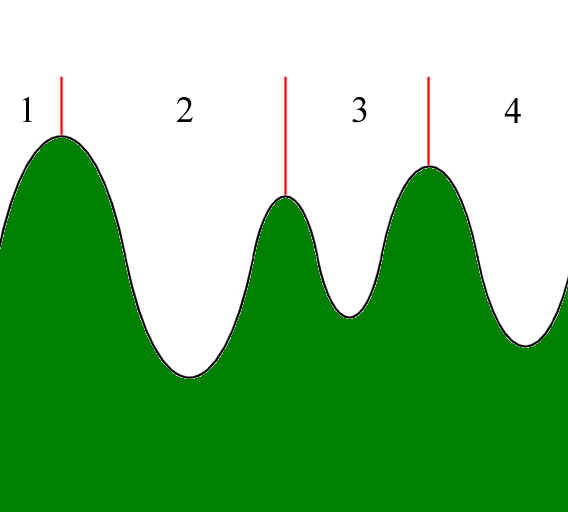
\includegraphics[width=.22\linewidth]{segmentation-watershed-floodingconcept-d.png}}%
\caption{The flooding concept of the watershed transform: (a) beginning the flooding; (b) two catchment basins meet; (c) building a watershed at the join point; (d) the division of the landscape into catchment basins.}
\label{fig:segmentation-watershed-floodingconcept}
\end{stusubfig}
%---

%---
\begin{stusubfig}{p}
	\subfigure[The input image]
	{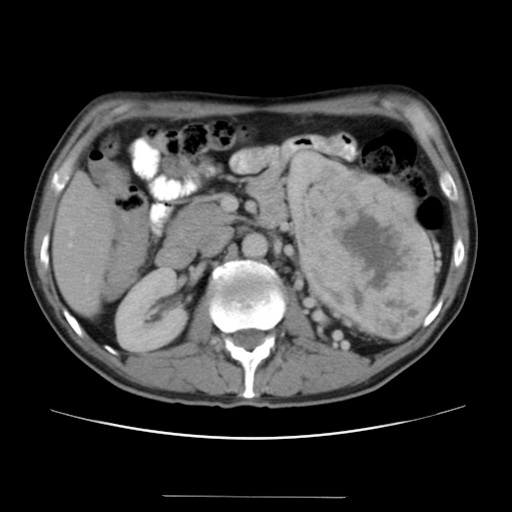
\includegraphics[height=5cm]{segmentation-watershed-adfexample-unsmoothed.png}}%
	%
	\hspace{4mm}%
	%
	\subfigure[The watershed of the (gradient magnitude of the) image]
	{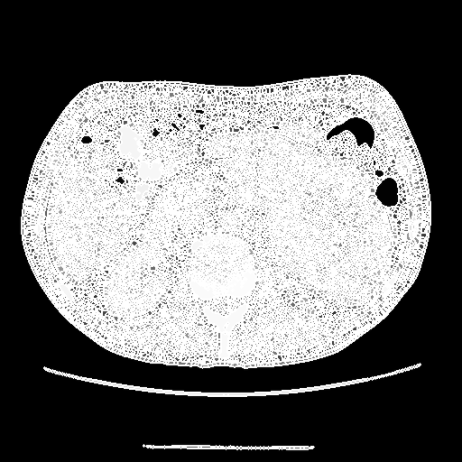
\includegraphics[height=5cm]{segmentation-watershed-adfexample-unsmoothedws.png}}%
\caption{The effects of the watershed transform. Note that the output is heavily over-segmented because the input is not smooth.}
\label{fig:segmentation-watershed-adfexample}
\end{stusubfig}
%---

\noindent Image-based watershed methods produce a partition of their input into regions (see Figure~\ref{fig:segmentation-watershed-adfexample}). This can then be used for further processing.

\subsection{The Waterfall Transform}

In contexts where its input is not smooth, the watershed has a well-known tendency to produce an over-segmented output (again, see Figure~\ref{fig:segmentation-watershed-adfexample}). This is due to the presence of large numbers of spurious local minima in the input -- in conceptual terms, we are effectively segmenting a pock-marked landscape. A wide variety of approaches exist to mitigate this problem:

\begin{itemize}

\item Pre-processing methods \cite{prochazka10,belaid09,meyer90,consularo07,gonzalez09,lotufo02b} transform the input to the watershed to reduce the number of spurious local minima. Various authors achieve this using noise reduction techniques, e.g.~anisotropic diffusion filtering \cite{perona90}, Gaussian blurring, median filtering or variants of the wavelet transform \cite{prochazka10}. Noise reduction is rarely enough to actually solve the problem on its own, but is often a helpful pre-cursor to applying hierarchical segmentation approaches -- note that this was done when producing Figure~\ref{fig:ipfs-ctconcept}, which is why the lowest partition of the image appears less over-segmented there than in Figure~\ref{fig:segmentation-watershed-adfexample}. Other authors make use of different definitions of the gradient that give greater weight to the main edges in the image, e.g.~\cite{belaid09} uses the topological gradient. Another popular approach is watershed-from-markers \cite{meyer90}, whereby the input is segmented into catchment basins associated with a fixed set of markers rather than with all of its local minima. Manual marker specification can directly tackle the oversegmentation problem by effectively specifying the desired number of output regions, but imposes a significant input burden on the user. As an alternative, various ways of automatically generating markers have been devised, e.g. \cite{consularo07} describes two approaches based on quadtrees and centroidal Voronoi diagrams and \cite{gonzalez09} describes an approach that generates markers by clustering the output regions of an initial, unconstrained watershed. Lotufo et al.\ \cite{lotufo02b} describe an algorithm that implicitly raises the image by a fixed amount, erodes it to remove insignificant minima (those whose catchment basins would have a smaller depth than the raising amount) and then passes the result (known as a morphological sup-reconstruction of the original image) through a normal watershed.

\item Post-processing methods \cite{bieniecki04,duarte05,frucci06,gies04,patino05,stawiaski08} directly reduce oversegmentation by merging together some of the regions output by the watershed, e.g.~\cite{gies04} describes a statistical approach to merging regions, \cite{patino05} groups similar regions using the composition of fuzzy relations and \cite{stawiaski08} merges regions using graph cuts. Bieniecki \cite{bieniecki04} describes a hybrid method that classifies the input image using a k-nearest neighbour approach and then removes watershed boundaries whose pixels all have the same class. Some post-processing methods (including, as we will see, the waterfall transform) merge regions in the output iteratively so as to construct a hierarchy of partitions of the input image. This does not reduce the over-segmentation of the lowest partition, but means instead that higher partitions may contain regions that are useful for later processing, e.g.~feature identification. (An interesting comparison can be drawn here with Felzenszwalb's algorithm \cite{felzenszwalb03}, a non-watershed approach that works by iteratively merging pairs of regions whose mutual difference is small compared to the amounts by which they differ internally. This is designed to run on a graph of the input image itself rather than the output of an initial watershed, and it takes more account of the internal properties of regions than the waterfall, but in many other ways the two share much in common.)

\end{itemize}
%
%---
\begin{stusubfig}{t}
	\subfigure[]
	{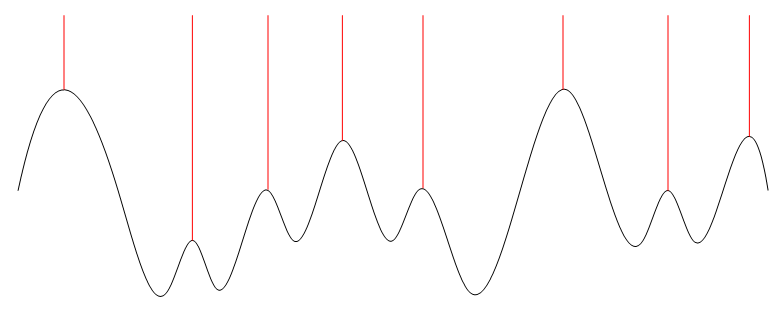
\includegraphics[height=2cm]{segmentation-waterfall-passconcept-a.png}}%
	%
	\hspace{4mm}%
	%
	\subfigure[]
	{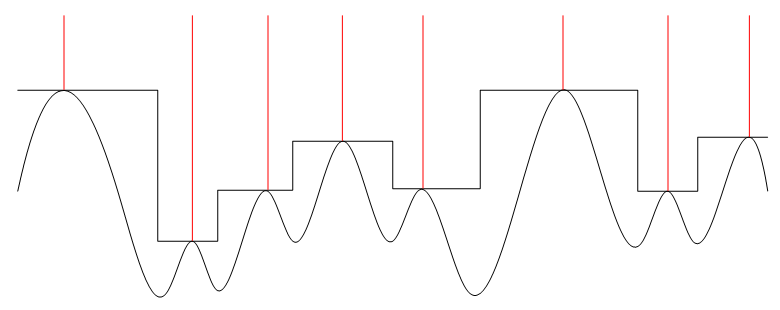
\includegraphics[height=2cm]{segmentation-waterfall-passconcept-b.png}}%
	%
	\hspace{4mm}%
	%
	\subfigure[]
	{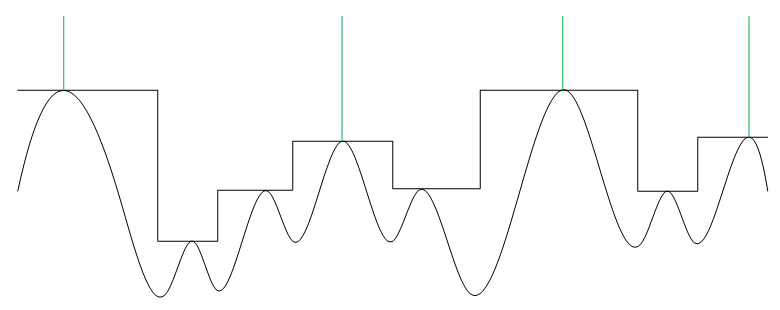
\includegraphics[height=2cm]{segmentation-waterfall-passconcept-c.png}}%
	%
	\hspace{4mm}%
	%
	\subfigure[]
	{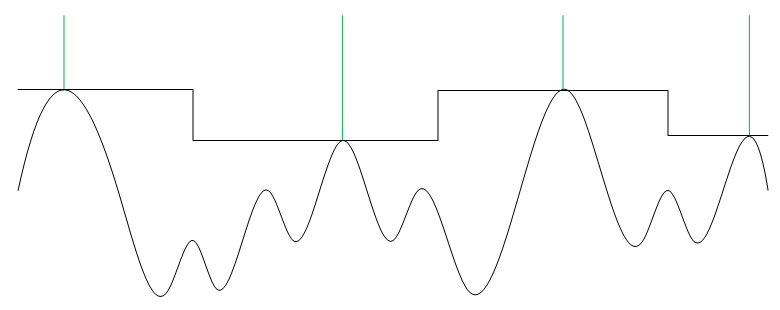
\includegraphics[height=2cm]{segmentation-waterfall-passconcept-d.png}}%
	%
	\hspace{4mm}%
	%
	\subfigure[]
	{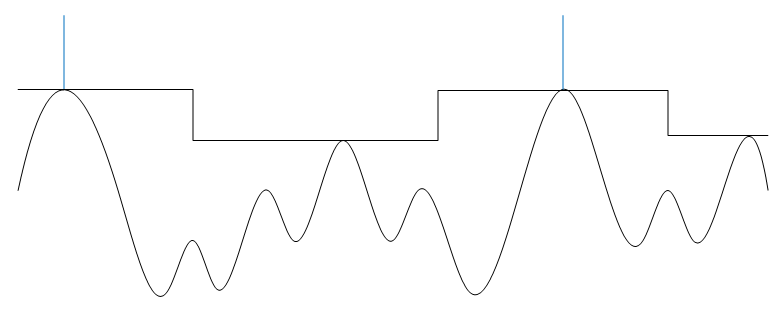
\includegraphics[height=2cm]{segmentation-waterfall-passconcept-e.png}}%
\caption{A conceptual view of the waterfall transform: (a) the initial partition output by the watershed; (b) after transforming it into a stepped landscape; (c) after performing a watershed transform on the stepped landscape; (d) after the second step transformation; (e) after performing another watershed transform.}
\label{fig:segmentation-waterfall-passconcept}
\end{stusubfig}
%---
%
The waterfall transform itself is a multi-pass, hierarchical post-processing method for the watershed. Its hierarchical nature is an advantage for the purposes of later feature identification, because the hierarchy it produces provides a helpful space in which to search for image features at different scales. As shown in Figure~\ref{fig:ipfs-ctconcept}, it generates a sequence of partitions of a landscape, each coarser (i.e.~containing fewer regions) than the one preceding it. Conceptually, each pass of the waterfall takes its input partition (Figure~\ref{fig:segmentation-waterfall-passconcept}(a)) and transforms it into a `stepped' landscape, where there is a step corresponding to each watershed boundary, with the height of a lowest pass point along that boundary (Figure~\ref{fig:segmentation-waterfall-passconcept}(b)). It then performs a watershed transform on this stepped landscape and outputs a coarser partition of the landscape as its result (Figure~\ref{fig:segmentation-waterfall-passconcept}(c)). This process can be repeated as long as the most recent partition has more than one catchment basin (Figures~\ref{fig:segmentation-waterfall-passconcept}(d) and (e)).

\subsection{Marcotegui's Method}

Whilst it is possible to perform the waterfall using the conceptual approach just described, repeatedly transforming the landscape can potentially be costly -- e.g.~image-based methods for the waterfall have to process all of the pixels in each region rather than just processing the region itself. This militates for alternative approaches to the waterfall based on graphs -- these can be more efficient because an entire region can be represented by a single node.

Marcotegui's method \cite{marcotegui05} is a fast and effective example of such an approach. It works on a minimum spanning tree (MST) of the (weighted) region adjacency graph (RAG) of its input partition\footnotemark{}. The nodes of this graph correspond to regions in the input partition; its edges join adjacent nodes, and each edge is weighted with the height of a lowest pass point on the boundary between the nodes it joins.

\footnotetext{The justification for why an MST is sufficient can be found in \cite{marcotegui05}.}

At the start of Marcotegui's method, the first input partition (produced from the gradient magnitude of the input using the watershed transform) is converted into its RAG representation and an MST is built from the RAG (see \S{}A.2 of \cite{golodetz11} for implementation details). This MST is then subjected to a sequence of waterfall passes. Each waterfall pass performs a flooding-based watershed on the MST to decide which regions should be merged and contracts appropriate edges in the MST to effect this (contracting an edge means combining the nodes at either end of the edge and removing the edge itself from the MST)\footnotemark{}. In detail, this involves the following steps:

\footnotetext{It should be noted that the use of edge contraction to merge regions in graph-based image segmentation algorithms is a ubiquitous technique that is by no means restricted to the waterfall (e.g.~see \cite{lezoray12}), since it is more efficient to simply merge together two nodes in a graph than to combine the two regions they represent by e.g.~unioning sets of pixels.}

%---
\begin{stusubfig}{p}
	\subfigure[]
	{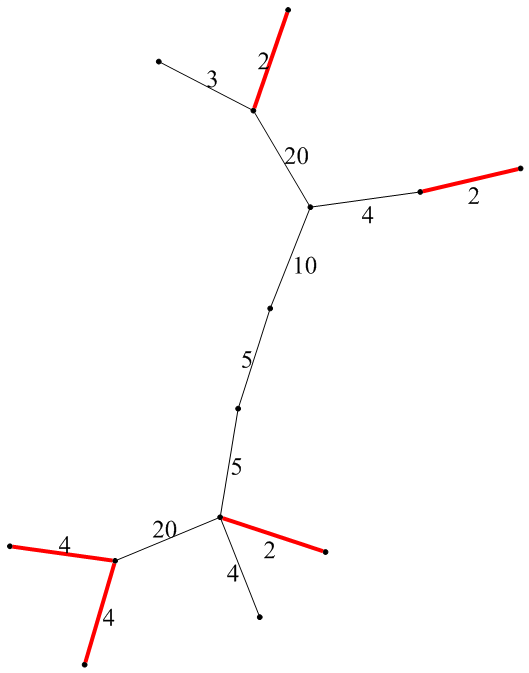
\includegraphics[width=.32\linewidth]{segmentation-waterfall-marcotegui-graphlocalminima.png}}%
	%
	\hspace{4mm}%
	%
	\subfigure[]
	{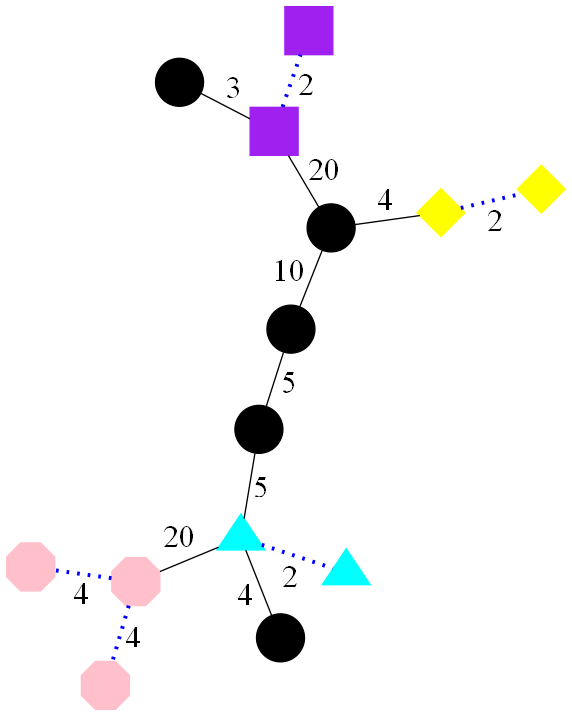
\includegraphics[width=.32\linewidth]{segmentation-waterfall-marcotegui-localminimaelision.png}}%	
\caption{Finding and contracting a graph's local minima for Marcotegui's method: (a) the graph from \cite{marcotegui05} and its local minima (drawn in red/dashed); (b) contracting/colouring the local minima (the edges to be contracted are drawn in blue/dotted).}
\label{fig:segmentation-waterfall-marcotegui-localminima}
\end{stusubfig}
%---

%---
\begin{stusubfig}{p}
	\subfigure[Initial state]
	{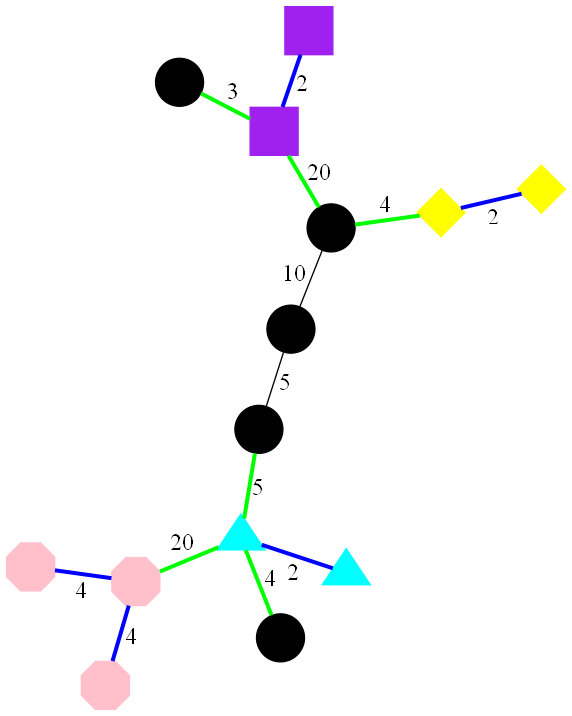
\includegraphics[width=.3\linewidth]{segmentation-waterfall-marcotegui-propagation-a.png}}%
	%
	\hspace{4mm}%
	%
	\subfigure[Contract the 3 edge]
	{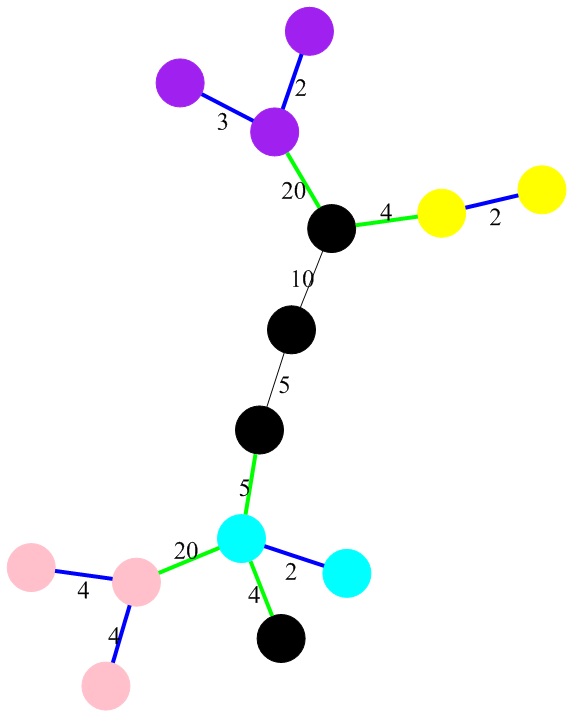
\includegraphics[width=.3\linewidth]{segmentation-waterfall-marcotegui-propagation-b.png}}%
	%
	\hspace{4mm}%
	%
	\subfigure[Contract a 4 edge]
	{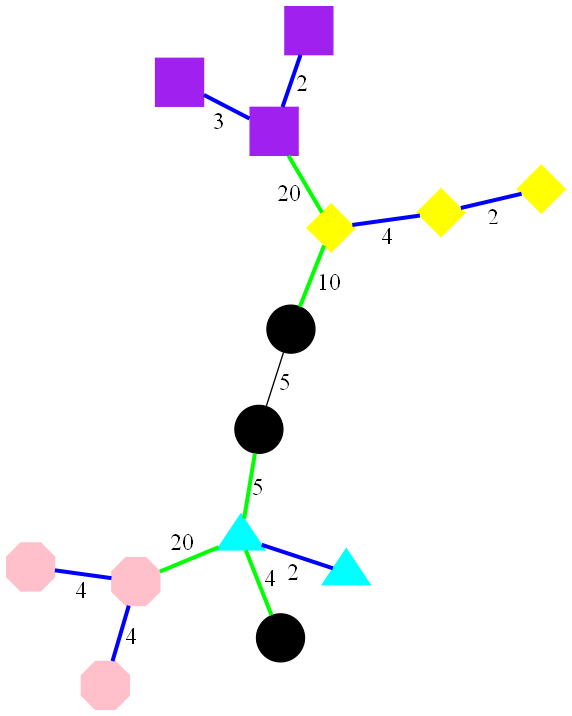
\includegraphics[width=.3\linewidth]{segmentation-waterfall-marcotegui-propagation-c.png}}%
	%
	\hspace{4mm}%
	%
	\subfigure[Contract another 4 edge]
	{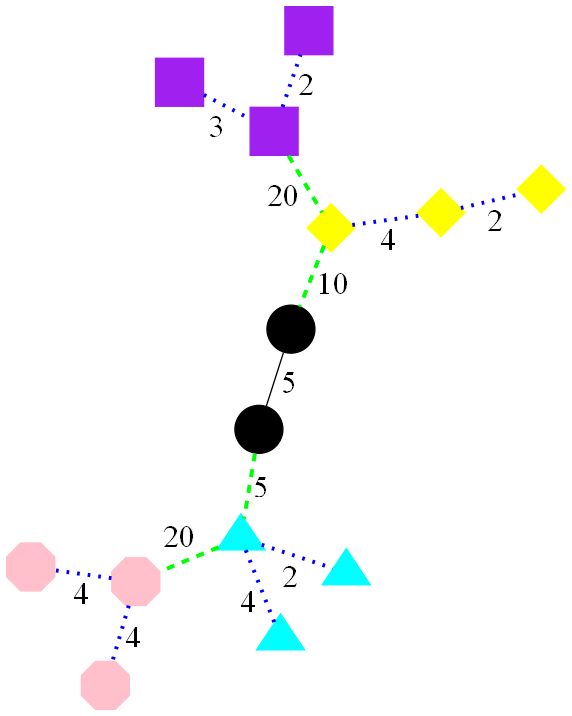
\includegraphics[width=.3\linewidth]{segmentation-waterfall-marcotegui-propagation-d.png}}%
	%
	\hspace{4mm}%
	%
	\subfigure[Contract the 5 edge]
	{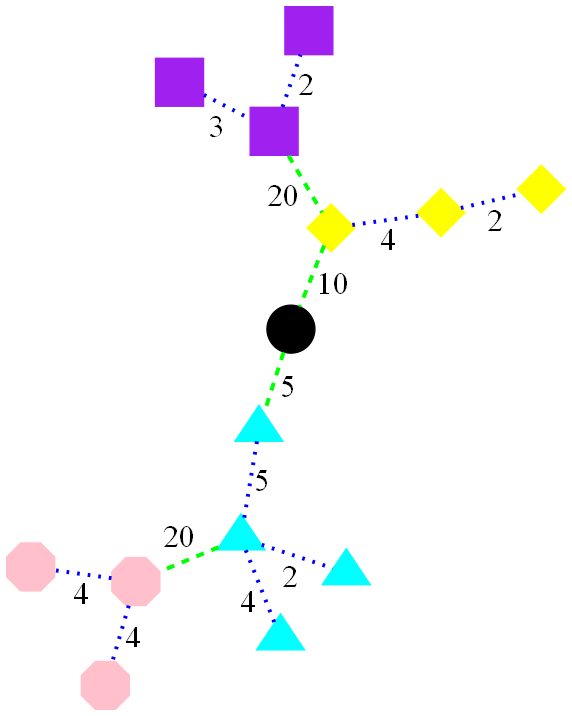
\includegraphics[width=.3\linewidth]{segmentation-waterfall-marcotegui-propagation-e.png}}%
	%
	\hspace{4mm}%
	%
	\subfigure[Contract another 5 edge]
	{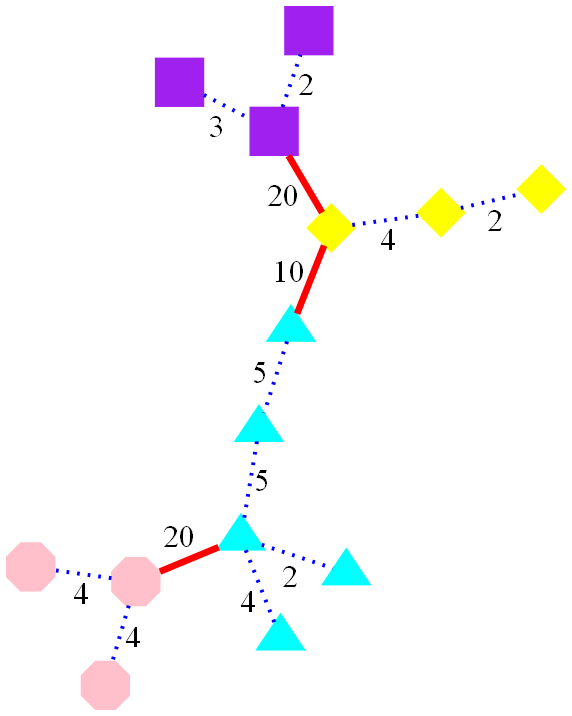
\includegraphics[width=.3\linewidth]{segmentation-waterfall-marcotegui-propagation-f.png}}%
\caption{The propagation step of Marcotegui's method, illustrated on the graph in \cite{marcotegui05}: blue/dotted edges have already been contracted, green/dashed edges are under consideration, and red edges will not be contracted.}
\label{fig:segmentation-waterfall-marcotegui-propagation}
\end{stusubfig}
%---

\begin{enumerate}

\item \emph{Determination of the local minima of the MST.} A local minimum of a weighted graph $G$ is a connected subgraph of $G$ whose edges have equal weight and whose adjacent edges in $G$ have strictly higher weights. Figure~\ref{fig:segmentation-waterfall-marcotegui-localminima}(a) shows an example graph and its local minima. Algorithmically, we iterate over the edges in the MST and flood out from each one to determine (i) whether it's part of a local minimum and (ii) the extent of the minimum if so.

\item \emph{Contraction of the local minima.} This is equivalent to merging minimal plateaux in a landscape into single points to which water runs down. See Figure~\ref{fig:segmentation-waterfall-marcotegui-localminima}(b). For clarity, we represent contraction in the figures by assigning the nodes at the ends of a contracted edge the same colour rather than removing the edge itself.

\item \emph{Propagation.} We flood out from the nodes that now represent the local minima (`marker nodes') along the edges, in non-decreasing order of edge weight, starting from the edges directly adjacent to the marker nodes. Each edge will either join a marker to another marker, in which case it should be ignored (since contracting it would merge two catchment basins), or it will join a marker to a non-marker, in which case it should be contracted. See Figure~\ref{fig:segmentation-waterfall-marcotegui-propagation}.

\end{enumerate}

\noindent It is important to note that the order in which edges should be processed during the propagation step is not well-defined (note that multiple edges can have the same weight and thus be candidates for contraction simultaneously). A straightforward implementation of the propagation step would use a priority queue and pop a lowest adjacent edge for consideration each time: thus the next edge to be considered ends up depending fundamentally on the way the priority queue is implemented. The consequence of this is that non-minimal plateaux in the MST are handled in a rather arbitrary way. This is not necessarily a problem in practice -- there tend to be only a small number of non-minimal plateaux in most realistic MSTs, so it doesn't seriously affect the end result -- but it still seems undesirable to have the segmentation output depend so closely on the implementation of an internal data structure which may in principle be subject to change. This issue is dealt with in \S\ref{sec:golodetz}.

%############################
\section{The Simplified Waterfall (SW) Method}
\label{sec:nicholls}
%############################

Despite the speed and effectiveness of Marcotegui's method, it can be somewhat intricate to implement \cite{golodetz08} because it is defined as a general graph method even though it operates on a tree. A simpler, tree-based method can be devised by observing that if an edge is not contracted by a waterfall pass, it is because it is a highest edge separating two adjacent catchment basins (alternatively, it is a highest edge on the MST path between two adjacent local minima in the MST). Instead of explicitly finding the local minima in the graph and flooding out from them, it therefore suffices to root the MST somewhere and then work recursively up from the bottom of the tree, carefully maintaining a highest edge (`guard edge') guarding each local minimum encountered on the way.

%---
\begin{stusubfig}{p}
	\subfigure[Before rooting the MST]
	{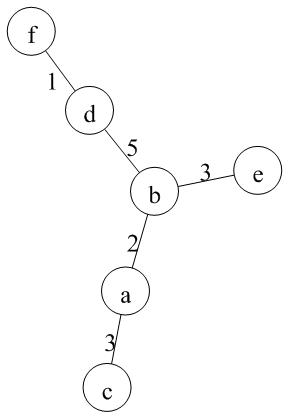
\includegraphics[height=5.5cm]{segmentation-waterfall-nicholls-root-before.png}}%
	%
	\hspace{4mm}%
	%
	\subfigure[After rooting it]
	{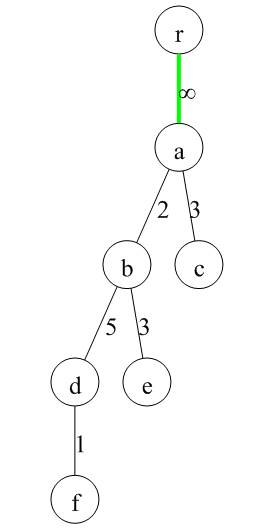
\includegraphics[height=5.5cm]{segmentation-waterfall-nicholls-root-after.png}}%
\caption{The SW method starts by picking a node at which to root the MST}% and adding a dummy root edge above the chosen root}
\label{fig:segmentation-waterfall-nicholls-root}
\end{stusubfig}
%---

%---
\begin{stusubfig}{p}
	\subfigure[The considered edge is a lowest edge]
	{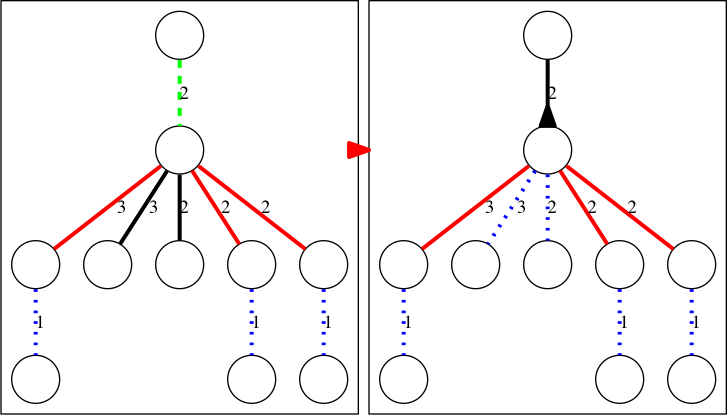
\includegraphics[height=4.5cm]{segmentation-waterfall-nicholls-cases-b.png}}%
	%
	\hspace{4mm}%
	%
	\subfigure[The considered edge is not a lowest edge]
	{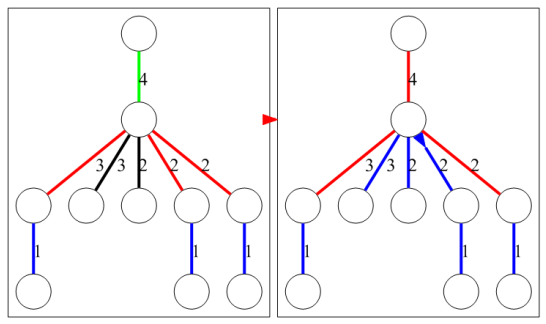
\includegraphics[height=4.5cm]{segmentation-waterfall-nicholls-cases-a.png}}%
\caption[Case analysis for step 2(c) of the SW method]{Case analysis for step 2(c) of the SW method: black edges are non-guards, red edges are guards, blue/dotted edges are those which have been contracted and the green/dashed edge is $e = (n_p,n_c)$, the edge under active consideration. The arrow (on the node $n_c$) indicates the direction in which the method presumes water to flow.}
\label{fig:segmentation-waterfall-nicholls-cases}
\end{stusubfig}
%---

%---
\begin{stusubfig}{p}
	\subfigure[Level 7]{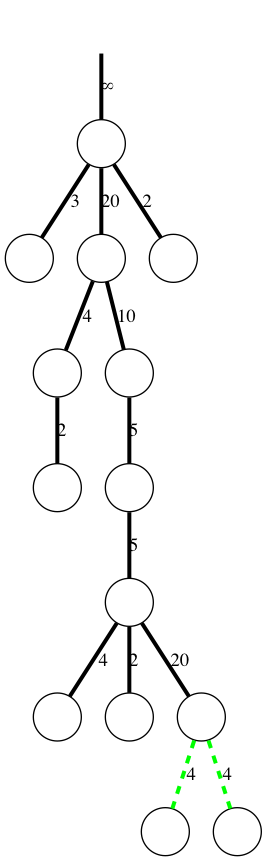
\includegraphics[width=.2\linewidth]{segmentation-waterfall-nicholls-example-a.png}}%
	\hspace{4mm}%
	\subfigure[Level 6]{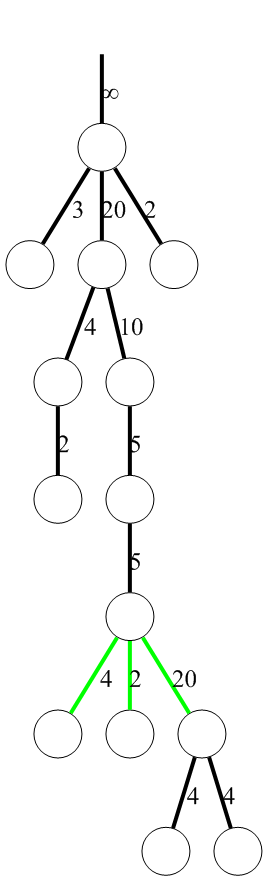
\includegraphics[width=.2\linewidth]{segmentation-waterfall-nicholls-example-b.png}}%
	\hspace{4mm}%
	\subfigure[Level 5]{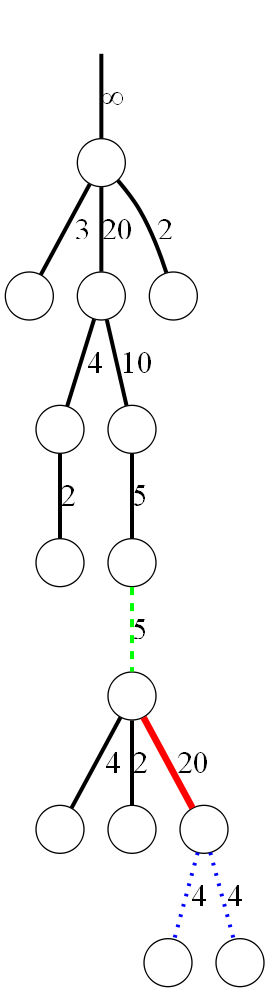
\includegraphics[width=.2\linewidth]{segmentation-waterfall-nicholls-example-c.png}}%
	\hspace{4mm}%
	\subfigure[Level 4]{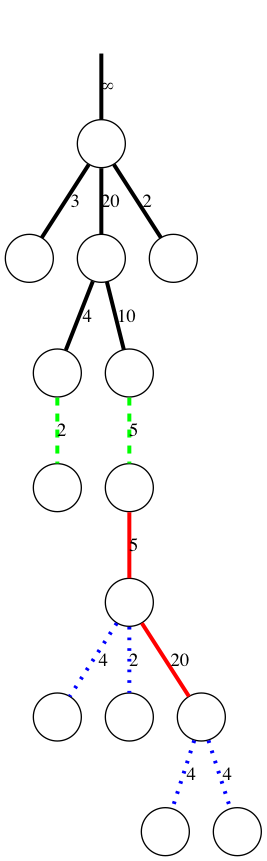
\includegraphics[width=.2\linewidth]{segmentation-waterfall-nicholls-example-d.png}}%
	\\
	\subfigure[Level 3]{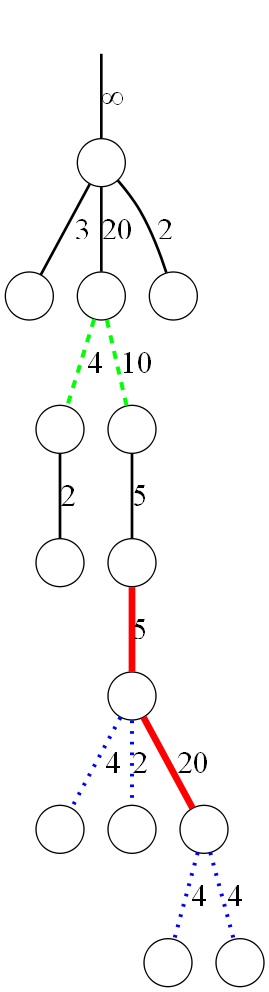
\includegraphics[width=.2\linewidth]{segmentation-waterfall-nicholls-example-e.png}}%
	\hspace{4mm}%
	\subfigure[Level 2]{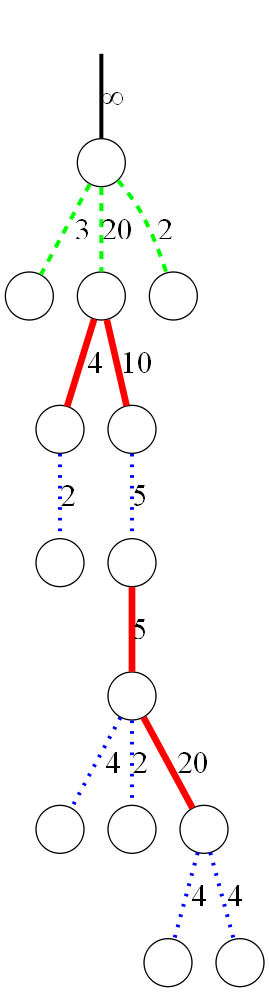
\includegraphics[width=.2\linewidth]{segmentation-waterfall-nicholls-example-f.png}}%
	\hspace{4mm}%
	\subfigure[Level 1]{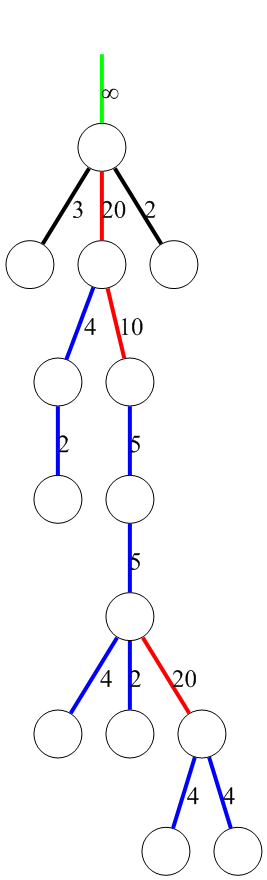
\includegraphics[width=.2\linewidth]{segmentation-waterfall-nicholls-example-g.png}}%
	\hspace{4mm}%
	\subfigure[Result]{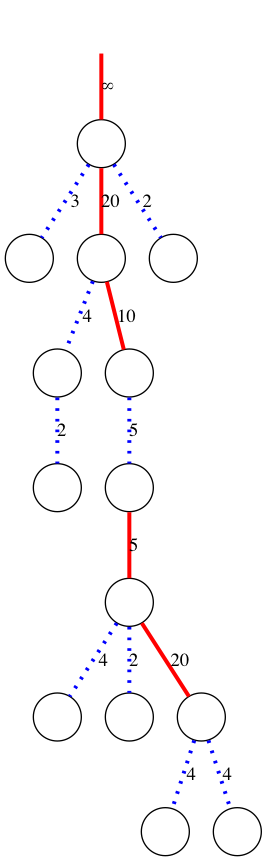
\includegraphics[width=.2\linewidth]{segmentation-waterfall-nicholls-example-h.png}}%
\caption[The SW method in action]{The SW method in action (considering all the edges in each level at a time for space reasons): black edges are non-guards, red edges are guards, blue/dotted edges are those which have been contracted and green/dashed edges are ones under active consideration. Note that in this example, the SW method's treatment of non-minimal plateaux has resulted in a $5$ edge being retained when it would have been contracted by Marcotegui's method.}
\label{fig:segmentation-waterfall-nicholls-example}
\end{stusubfig}
%---

The Simplified Waterfall (SW) method initially roots the MST (see Figure~\ref{fig:segmentation-waterfall-nicholls-root}), adding a dummy `root edge' with a weight strictly greater than the weights of the edges descending from the root node (we will henceforth -- without ambiguity -- call edges descending from a node \emph{children} of the edge ascending from that node). The weight chosen is unimportant, but $\infty$ or $1$ greater than the maximum weight on a child edge are sensible choices (we use $\infty$ here for clarity of presentation).

To specify the method, let $T = (N,E)$ be the rooted MST on which the method is to operate, with node set $N = (n_i)$ and edge set $E = \{(n_p,n_c)\}$ such that $n_p$ is the parent of $n_c$. We define $C(e)$ to be the children of edge $e$ in some unspecified but fixed order, i.e.
%
\[
C(e) = (c_1,...,c_k) = ((n_c,n') \in E \; | \; e = (n_p,n_c))
\]
%
Each edge $e$ has an immutable weight $w(e) \in \mathbb{N}^+$ and a mutable flag $f(e) \in \{\mathcal{G},\mathcal{NG}\}$, where $f(e) = \mathcal{G}$ denotes that $e$ is a guard edge and $f(e) = \mathcal{NG}$ denotes that it is a non-guard. The root edge is denoted $e_r$ and satisfies $w(e_r) = \infty$, as mentioned above.

Each pass of the method is then invoked on $e_r$ and proceeds recursively as follows (in which we denote the current edge, initially $e_r$, as $e$):
%
\begin{enumerate}

\item If $e$ is a leaf edge (i.e.~$C(e) = \emptyset$), then it is marked as a non-guard edge (i.e.~$f(e) \leftarrow \mathcal{NG}$).

\item Otherwise:

\begin{enumerate}

\item We recurse on all the children of $e$ (i.e.~the edges in $C(e)$).

\item A child edge $c_{\min}$ with minimum weight is chosen (if one or more of the children with minimum weight is a guard edge, one of those is chosen in preference to a non-guard). Formally, let $\mbox{SC}(e)$ be a possible result of sorting $C(e)$ first by weight (in non-decreasing order) and then by flag ($\mathcal{G}$ before $\mathcal{NG}$), and let $\pi_1,...,\pi_k$ be the corresponding permutation of $1,...,k$, i.e.
%
\[
SC(e) = (c_{\pi_1},...,c_{\pi_k})
\]
%
Then $c_{\min}$ is chosen to be $c_{\pi_1}$. Note that $c_{\min}$ is not uniquely specified because there may be more than one possible way of sorting $C(e)$ to produce $\mbox{SC}(e)$.

\item There are now two possibilities. If $w(e) \le w(c_{\min})$\footnotemark{}, i.e.~the current edge $e = (n_p,n_c)$ is one of the lowest edges leading out of its child node $n_c$, then at least part of the implied flow from $n_c$ is along $e$ (see Figure~\ref{fig:segmentation-waterfall-nicholls-cases}(a)), in which case we mark $e$ as a non-guard edge (i.e.~$f(e) \leftarrow \mathcal{NG}$). Conversely, if $w(e) > w(c_{\min})$ then none of the implied flow from the node is along $e$ and at least part of it is along $c_{\min}$ (see Figure~\ref{fig:segmentation-waterfall-nicholls-cases}(b)), in which case we mark $e$ as a guard (i.e.~$f(e) \leftarrow \mathcal{G}$) and $c_{\min}$ as a non-guard (i.e.~$f(c_{\min}) \leftarrow \mathcal{NG}$). Note that in both cases, the method arbitrarily assumes that all of the implied flow is along a single edge leading out of $n_c$, even though there may be multiple edges leading out of $n_c$ that share the same lowest weight.

\item All non-guard children (i.e.~$\{c \in C(e) \; | \; f(c) = \mathcal{NG}\}$) are then contracted.

\end{enumerate}

\end{enumerate}
%
Figure~\ref{fig:segmentation-waterfall-nicholls-example} illustrates how the method works on the same graph used to illustrate Marcotegui's method above (particular attention is drawn to the handling of the non-minimal plateau containing two edges with weight $5$). The assumption that all of the implied flow from a node is along a single edge is this method's way of dealing with non-minimal plateaux in the MST. As with the Marcotegui method's dependence on a priority queue implementation, this is a slightly arbitrary way of handling non-minimal plateaux: in particular, the selected direction of implied flow from a particular node depends on both where the MST is rooted and the way in which $C(e)$ is sorted when choosing $c_{\min}$. All of this affects which specific edges are contracted. As with Marcotegui's method, this tends not to significantly degrade the end result, but it still in principle seems desirable to devise a method that does not depend on such implementation details. In the following section, we therefore present an alernative tree-based method that handles non-minimal plateaux in the MST more robustly.

\footnotetext{As an interesting aside, we also investigated the use of the condition $w(e) < w(c_{\min})$ here as an alternative. This leads to a different version of the Simplified Waterfall that is in general less robust in its treatment of non-minimal plateaux than the version described in this paper. We focus on the primary version here since it yields more reliable results.}

%#############################
\section{The Balanced Waterfall (BW) Method}
\label{sec:golodetz}
%#############################

In order to account for non-minimal plateaux in the MST, we adopt an idea from Meijster and Roedink's image watershed algorithm \cite{meijster98}: if we transform the landscape to make it `lower-complete' (that is, we transform it into a landscape in which there is a unique path of steepest descent from each point), then the direction of flow is clear at every point and there is no ambiguity about how to assign non-minimal plateau points to catchment basins. The method for making the image lower-complete described in \cite{meijster98} has the effect of treating pixels that are further from the border of a plateau as being in some sense `higher' than those on the boundary. The same sort of idea can be applied in the context of a waterfall pass (although it is not necessary to actually transform the MST to make it lower-complete): where there are non-minimal plateaux in the MST, we can arrange to treat the nodes further from the border of the plateaux as being `higher' than their boundary counterparts. As we will see, this enables a robust decision to be made about which edges to contract.

The Balanced Waterfall (BW) method is a tree-based, rainfalling approach and works in three recursive sub-passes. The first sub-pass works up the tree from the leaf nodes, marking initial path(s) of steepest descent from each node whilst allowing for the fact that they may need to be refined later. The second sub-pass works down the tree from the root, updating the path(s) for each node to take account of routes via parent edges and marking edges for later contraction as necessary. The final sub-pass works up the tree again to actually contract the marked edges (this cannot be done on a down pass for technical reasons). The MST can be rooted anywhere in order to form the input tree -- the results are the same for any choice of root.

To specify the method, let $T = (N,E)$ again be the rooted MST on which the method is to operate (this time without the dummy root edge added by the SW method). We define $C_N(n)$ to be the child nodes of node $n$, i.e.~$\{n_c \; | \; \exists (n,n_c) \in E\}$, $C_E(n)$ to be the child edges of $n$, i.e.~$\{(n,n_c) \; | \; n_c \in C_N(n)\}$ and $p_N(n)$ and $p_E(n)$ to be the corresponding parent functions, e.g.~$n_c \in C_N(n) \Leftrightarrow n = p_N(n_c)$. Edges have immutable weights in $\mathbb{N}^+$, as for the previous method. Each node $n$ has a distance value $d(n)$, a set of arrows $A(n)$ (each element of which is a node $n'$ indicating an arrow from $n$ to $n'$) and a flag $\funcname{checkParent}(n)$ (false by default), indicating whether or not to check for an upwards route from $n$ in step $2$ of the method. We additionally define the following helper functions: $\funcname{adjacentEdges}(n)$ determines the set of edges that have $n$ as an endpoint, $\funcname{farEnd}(e,n)$ determines the node at the far end of edge $e$ from node $n$, and $\funcname{reverseArrow}(e,n)$ determines whether or not there is an arrow on the node at the far end of $e$ from $n$ that points towards $n$, i.e.~$n \in A(\funcname{farEnd}(e,n))$. For brevity, we also define a function $\funcname{farEnds}(E',n)$ that maps $\funcname{farEnd}$ over the edge set $E'$.

For each waterfall pass, the three sub-passes of the method are invoked sequentially on the root node $n_r$ of $T$ as follows (in which we consistently denote the current node, initially $n_r$ for each sub-pass, as $n$):

%---
\begin{stusubfig}{!t}
	\subfigure[]
	{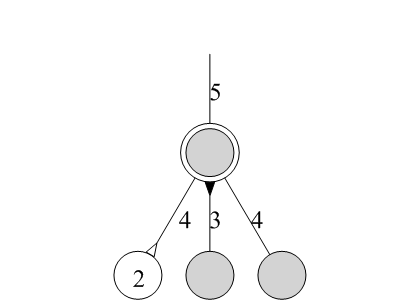
\includegraphics[width=.35\linewidth]{segmentation-waterfall-smg-pass1cases-a.png}}%
	%
	\hspace{4mm}%
	%
	\subfigure[]
	{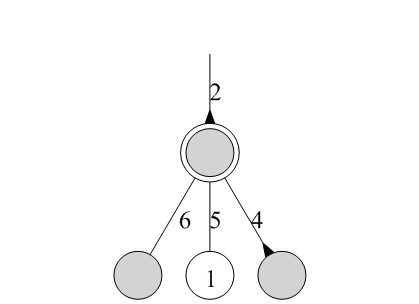
\includegraphics[width=.35\linewidth]{segmentation-waterfall-smg-pass1cases-b.png}}%
	%
	\hspace{4mm}%
	%
	\subfigure[]
	{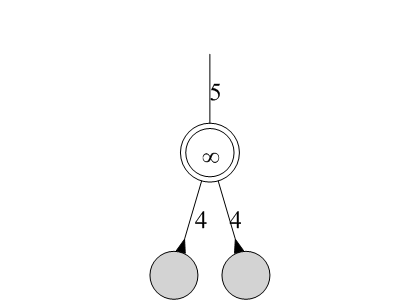
\includegraphics[width=.35\linewidth]{segmentation-waterfall-smg-pass1cases-e.png}}%
	%
	\hspace{4mm}%
	%
	\subfigure[]
	{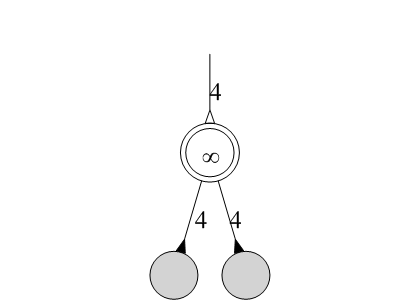
\includegraphics[width=.35\linewidth]{segmentation-waterfall-smg-pass1cases-f.png}}%
	%
	\hspace{4mm}%
	%
	\subfigure[]
	{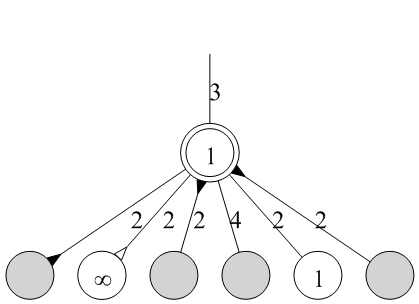
\includegraphics[width=.35\linewidth]{segmentation-waterfall-smg-pass1cases-c.png}}%
	%
	\hspace{4mm}%
	%
	\subfigure[]
	{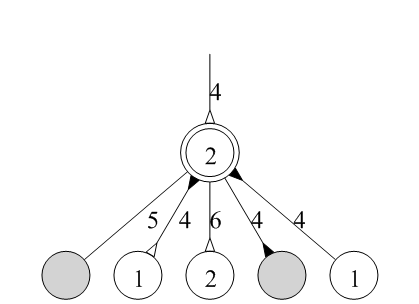
\includegraphics[width=.35\linewidth]{segmentation-waterfall-smg-pass1cases-d.png}}%
\caption{Case analysis for the first sub-pass of the BW method: (a) the node has a unique path of steepest descent down a child edge; (b) the node has a unique path of steepest descent up the parent edge; (c) there is no flow out of the node; (d) there is no downwards flow out of the node (but the parent edge still needs to be considered); (e) the node has more than one path of steepest descent (and the parent edge is not one of them); (f) the node has more than one \emph{downwards} path of steepest descent (but the parent edge still needs to be considered).}
\label{fig:segmentation-waterfall-smg-pass1cases}
\end{stusubfig}
%---

%---
\begin{stusubfig}{!t}
	\subfigure[The arrow from the parent node points towards us]
	{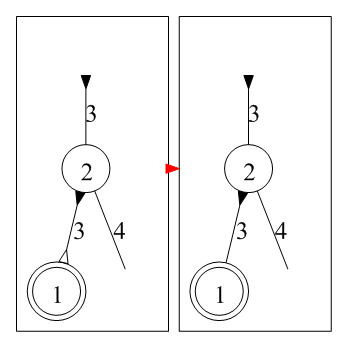
\includegraphics[height=4cm]{segmentation-waterfall-smg-resolutioncases-a.png}}%
	%
	\hspace{4mm}%
	%
	\subfigure[There is a better route via the parent node]
	{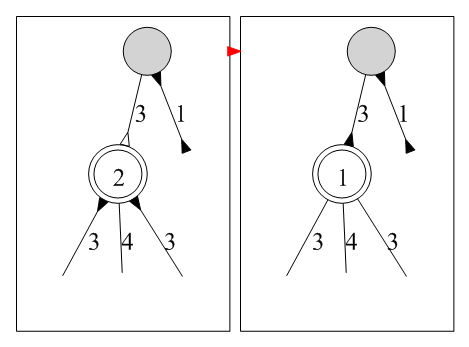
\includegraphics[height=4cm]{segmentation-waterfall-smg-resolutioncases-d.png}}%
	%
	\hspace{4mm}%
	%
	\subfigure[There is an equally good route via the parent node]
	{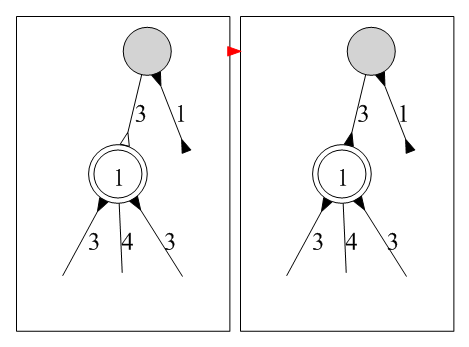
\includegraphics[height=4cm]{segmentation-waterfall-smg-resolutioncases-c.png}}%
	%
	\hspace{4mm}%
	%
	\subfigure[There is no flow from the parent node]
	{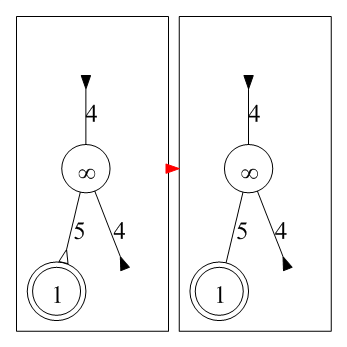
\includegraphics[height=4cm]{segmentation-waterfall-smg-resolutioncases-b.png}}%
\caption[Case analysis for step 2(a) of the BW method]{Case analysis for step 2(a) of the BW method (the circled node is the one currently under consideration in each case)}
\label{fig:segmentation-waterfall-smg-resolutioncases}
\end{stusubfig}
%---

%---
\begin{stusubfig}{p}
	\subfigure[UI/UI]{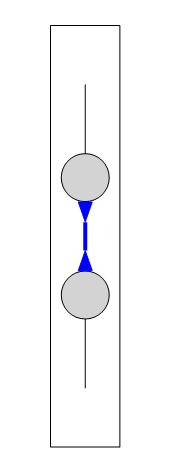
\includegraphics[height=5cm]{segmentation-waterfall-smg-mergecases-uiui.png}}%
	\hspace{4mm}
	\subfigure[UI/UO]{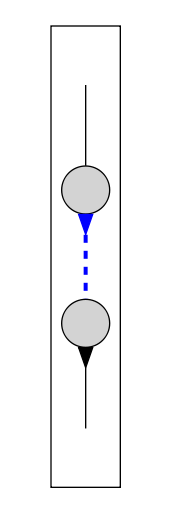
\includegraphics[height=5cm]{segmentation-waterfall-smg-mergecases-uiuo.png}}%
	\hspace{4mm}
	\subfigure[UI/AO]{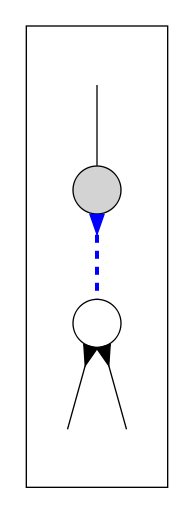
\includegraphics[height=5cm]{segmentation-waterfall-smg-mergecases-uiao.png}}%
	\hspace{4mm}
	\subfigure[UI/NF]{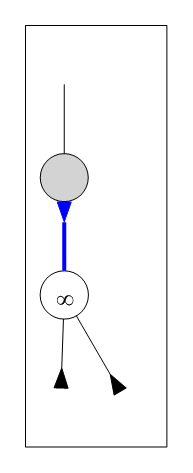
\includegraphics[height=5cm]{segmentation-waterfall-smg-mergecases-uinf.png}}%
	\hspace{4mm}
	\subfigure[NF/NF]{\includegraphics[height=5cm]{segmentation-waterfall-smg-mergecases-nfnf.png}}%
	\\
	\subfigure[UO/UO]{\includegraphics[height=5cm]{segmentation-waterfall-smg-mergecases-uouo.png}}%
	\hspace{4mm}
	\subfigure[UO/AI]{\includegraphics[height=5cm]{segmentation-waterfall-smg-mergecases-uoai.png}}%
	\hspace{4mm}
	\subfigure[UO/AO]{\includegraphics[height=5cm]{segmentation-waterfall-smg-mergecases-uoao.png}}%
	\hspace{4mm}
	\subfigure[UO/NF]{\includegraphics[height=5cm]{segmentation-waterfall-smg-mergecases-uonf.png}}%
	\\
	\subfigure[AO/AI]{\includegraphics[height=5cm]{segmentation-waterfall-smg-mergecases-aoai.png}}%
	\hspace{4mm}
	\subfigure[AO/AO]{\includegraphics[height=5cm]{segmentation-waterfall-smg-mergecases-aoao.png}}%
	\hspace{4mm}
	\subfigure[NF/AI]{\includegraphics[height=5cm]{segmentation-waterfall-smg-mergecases-nfai.png}}%
	\hspace{4mm}
	\subfigure[NF/AO]{\includegraphics[height=5cm]{segmentation-waterfall-smg-mergecases-nfao.png}}%
\caption[Case analysis for step 2(b) of the BW method]{Case analysis for step 2(b) of the BW method (a blue/dashed edge indicates that the edge would be contracted; a red/solid edge indicates that it wouldn't). The labels are AI = ambiguously in, AO = ambiguously out, NF = no flow, UI = unambiguously in and UO = unambiguously out.}
\label{fig:segmentation-waterfall-smg-mergecases}
\end{stusubfig}
%---

%---
\begin{stusubfig}{!t}
	\subfigure[The initial tree]{\includegraphics[width=.25\linewidth]{segmentation-waterfall-smg-example-initial.png}}%
	\hspace{4mm}%
	\subfigure[After step $1$]{\includegraphics[width=.25\linewidth]{segmentation-waterfall-smg-example-pass1.png}}%
	\hspace{4mm}%
	\subfigure[After step $2$]{\includegraphics[width=.25\linewidth]{segmentation-waterfall-smg-example-pass2.png}}%
\caption[The BW method running on a real example]{The BW method running on a real example: the arrows on the nodes indicate the flow direction, blue/dashed edges are those that will be contracted and red/bold edges are those that won't be.}
\label{fig:segmentation-waterfall-smg-example}
\end{stusubfig}
%---

\begin{enumerate}

\item \emph{Up Sub-Pass.}

\begin{enumerate}
\item We recursively process any children of the node (i.e.~any nodes in $C_N(n)$). The fact that the children are processed first is why this is called an `up' sub-pass.

\item If $n$ has a unique edge of steepest descent (i.e.~a unique lowest-weighted edge leading out of it, which can be the parent edge), add an arrow on the node pointing along the edge (see Figures~\ref{fig:segmentation-waterfall-smg-pass1cases}(a) and (b)). Formally, we define a set containing the lowest-weighted edges leading out of $n$:
%
\[
\funcname{steepestEdges}(n) = \argmin_{}\{w(e) \; | \; e \in \funcname{adjacentEdges}(n)\}
\]
%
Then if $\funcname{steepestEdges}(n) = \{e\}$, we set $A(n)$ to be $\{\funcname{farEnd}(e,n)\}$.

\item Otherwise, consider all the lowest-weighted child edges (i.e.~ignore the parent for now, even if it is also a lowest-weighted edge) that satisfy the condition that there is no arrow on the node at the other end of the edge pointing along the edge towards $n$. Formally, we define the set $\funcname{escapableChildEdges}(n)$ of such edges as:
%
\[
\{e \in \funcname{steepestEdges}(n) \backslash \{p_E(n)\} \; | \; \neg \funcname{reverseArrow}(e,n)\}
\]
%
If there are no such child edges (i.e.~$\funcname{escapableChildEdges}(n) = \emptyset$), then $n$ is unescapable along a child edge and its distance value $d(n)$ should be set to $\infty$ (see Figures~\ref{fig:segmentation-waterfall-smg-pass1cases}(c) and (d)). Otherwise, we assign to each edge $e \in \funcname{escapableChildEdges}(n)$ a temporary distance value $d'(e) = 1 + d(\funcname{farEnd}(e,n))$, i.e.~a value $1$ greater than the value on the node at the other end of the edge. (The value on the far node will be $0$ for nodes from which there is a unique path of steepest descent, and non-zero otherwise.) We pick all the escapable child edges whose distance value is minimal and add arrows from $n$ pointing along them (these indicate the initial paths of steepest descent from $n$). We also store the minimum distance value as $d(n)$ (see Figures~\ref{fig:segmentation-waterfall-smg-pass1cases}(e) and (f)). Formally, we write
%
\[
A(n) \leftarrow \funcname{farEnds}(\argmin_{}\{d'(e) \; | \; e \in \funcname{escapableChildEdges}(n)\}, n)
\]
%
and
\[
d(n) \leftarrow \min_{}\{d'(e) \; | \; e \in \funcname{escapableChildEdges}(n)\}.
\]

\item Finally, if the parent edge of $n$ was a lowest-weighted edge (i.e.~$p_E(n) \in \funcname{steepestEdges}(n)$), then we set $\funcname{checkParent}(n)$ to true to mark the parent edge as a potential path of steepest descent for further processing in the second sub-pass (see Figures~\ref{fig:segmentation-waterfall-smg-pass1cases}(d) and (f), in which an open-headed arrow is used to mark the parent edge).
\end{enumerate}

\item \emph{Down Sub-Pass.}

\begin{enumerate}
\item \emph{Check upwards route.} If $n$ was marked as having a potential upwards path of steepest descent (i.e.~$\funcname{checkParent}(n)$ is true), we first check whether or not there is an arrow on the parent node $p_N(n)$ pointing down the edge to this node (given by $\funcname{reverseArrow}(p_E(n),n)$). If there is such an arrow (see Figure~\ref{fig:segmentation-waterfall-smg-resolutioncases}(a)), then $n$ is unescapable via its parent; otherwise, there is a possible route upwards with distance value $d' = 1 + d(p_N(n))$. This is compared to the cost of the best existing routes downwards from $n$ via child edges (stored as $d(n)$). If, as in Figure~\ref{fig:segmentation-waterfall-smg-resolutioncases}(b), the upwards route is strictly better (i.e.~$d' < d(n)$), then it replaces the downwards routes (i.e.~$A(n) \leftarrow \{p_N(n)\}$) and we update the distance value on the node to reflect the better route (i.e.~$d(n) \leftarrow d'$). If, as in Figure~\ref{fig:segmentation-waterfall-smg-resolutioncases}(c), the upwards route is equally good (i.e.~$d' = d(n)$), the parent edge is marked (i.e.~$A(n) \leftarrow A(n) \cup \{p_N(n)\}$) but no other changes are made. If the upwards route is worse (i.e.~$d' > d(n)$), it is simply ignored. An extreme example of this case, when there is no flow at all out of the parent node, is shown in Figure~\ref{fig:segmentation-waterfall-smg-resolutioncases}(d).

\item \emph{Check whether the parent edge $p_E(n)$ (if any) should be contracted.} The decision on whether or not to contract an edge is based on a classification of its two end nodes with respect to the edge itself (this is why it can only be done at this point in the method). Nodes can be classified into one of five types with respect to the edge: unambiguously in (the flow from the node goes only along this edge), ambiguously in (part, but not all, of the flow from the node goes along this edge), unambiguously out (the flow from the node goes along precisely one of the other edges leading out of it), ambiguously out (the flow from the node goes along at least two of the other edges leading out of it) and no flow (there is no flow from the node at all). Based on these classifications, the parent edge is either marked for contraction or not according to the case analysis shown in Figure~\ref{fig:segmentation-waterfall-smg-mergecases}. Note that there are only $13$ cases possible, rather than the expected $15$: \{ambiguously in, ambiguously in\} and \{ambiguously in, unambiguously in\} can never occur due to the way the method works.

\item \emph{Recurse on any children}.
\end{enumerate}

\item \emph{Up Sub-Pass.} Walk back up the tree to contract the marked edges.

\end{enumerate}

\noindent Figure~\ref{fig:segmentation-waterfall-smg-example} illustrates how the method works on the now familiar graph used to demonstrate the workings of the previous two waterfall approaches.

%######################
\section{Experiments}
\label{sec:experiments}
%######################

We implemented all three methods (Marcotegui, SW and BW) in \emph{millipede} \cite{millipede}, our software for 3D abdominal CT image segmentation, feature identification and visualisation. The way in which we implemented Marcotegui's method in \emph{millipede} was a refinement of our initial approach that we described in \cite{golodetz08} -- in particular, the new implementation of the step that finds the local minima in the MST uses the first two passes of the BW method as an edge classifier (the local minima are those edges classified as either \{unambiguously in, unambiguously in\}, \{unambiguously in, no flow\} or \{no flow, no flow\}). This is a more efficient way of finding the local minima than the flooding approach described in \cite{golodetz08}.

We performed three experiments to compare the methods: the first quantifies the extent to which the results produced by the new methods are similar to those produced by the existing state-of-the-art, the second investigates the performance and scalability of the methods, and the third highlights the differences in non-minimal plateaux behaviour between the methods.

\subsection{Similarity of Results}
\label{subsec:experiments-similarity}

In order to demonstrate that our new methods produce results that are similar to those of the existing state-of-the-art, we quantitatively compared the partition hierarchies output by all three methods on the publicly-available dataset of $151$ images proposed by Gulshan et al.\ \cite{gulshan10} (see Figure~\ref{fig:sheep} for an example result). This dataset was chosen because it was of a suitable size and provided an interesting variety of different images (it was originally compiled using images from the GrabCut dataset \cite{rother04}, the PASCAL VOC'09 segmentation challenge \cite{everingham09} and the alpha-matting dataset \cite{rhemann09}). Since the images in the dataset are in colour, we first converted them to greyscale using the ImageMagick \cite{imagemagick} command\footnotemark{}:
%
\begin{alltt}\begin{center}
convert <colour filename> -separate -average <greyscale filename>
\end{center}\end{alltt}
%
Each of the three methods was then used to produce a hierarchy of partitions for each greyscale image. In each case, the gradient magnitude of the input image was initially smoothed using anisotropic diffusion filtering \cite{perona90} and the first output partition was produced using our implementation of Meijster and Roerdink's watershed algorithm \cite{meijster98}.

\footnotetext{It bears noting in passing that there are many different ways of converting colour images to greyscale. Whilst the choice makes little difference for our purposes here, we chose this method, which computes $(r + g + b) / 3$, because it is intuitive and avoids biasing the result in favour of any particular colour channel.}

%---
\begin{stusubfig}{!t}
	\subfigure{\includegraphics[width=.3\linewidth]{sheep_2007_003593.png}}%
	\hspace{4mm}%
	\subfigure{\includegraphics[width=.3\linewidth]{sheep_2007_003593.png}}%
	\hspace{4mm}%
	\subfigure{\includegraphics[width=.3\linewidth]{sheep_2007_003593.png}}%
	\\
	\subfigure{\includegraphics[width=.3\linewidth]{sheep_2007_003593-partition-2-M.png}}%
	\hspace{4mm}%
	\subfigure{\includegraphics[width=.3\linewidth]{sheep_2007_003593-partition-2-NC.png}}%
	\hspace{4mm}%
	\subfigure{\includegraphics[width=.3\linewidth]{sheep_2007_003593-partition-2-G.png}}%
	\\
	\subfigure{\includegraphics[width=.3\linewidth]{sheep_2007_003593-partition-3-M.png}}%
	\hspace{4mm}%
	\subfigure{\includegraphics[width=.3\linewidth]{sheep_2007_003593-partition-3-NC.png}}%
	\hspace{4mm}%
	\subfigure{\includegraphics[width=.3\linewidth]{sheep_2007_003593-partition-3-G.png}}%
	\\
	\subfigure{\includegraphics[width=.3\linewidth]{sheep_2007_003593-partition-4-M.png}}%
	\hspace{4mm}%
	\subfigure{\includegraphics[width=.3\linewidth]{sheep_2007_003593-partition-4-NC.png}}%
	\hspace{4mm}%
	\subfigure{\includegraphics[width=.3\linewidth]{sheep_2007_003593-partition-4-G.png}}%
	\\
	\subfigure{\includegraphics[width=.3\linewidth]{sheep_2007_003593-partition-5-M.png}}%
	\hspace{4mm}%
	\subfigure{\includegraphics[width=.3\linewidth]{sheep_2007_003593-partition-5-NC.png}}%
	\hspace{4mm}%
	\subfigure{\includegraphics[width=.3\linewidth]{sheep_2007_003593-partition-5-G.png}}%
\caption{The results of the three waterfall methods for the \emph{sheep\_2007\_003593} image from the dataset of Gulshan et al.\ \cite{gulshan10}. Starting from the top, the rows show partitions $0$, $2$, $3$, $4$ and $5$ of the image for each method (partition $1$, i.e.~the watershed result, is irrelevant and therefore not shown). The first column shows the results of Marcotegui's method, the second column shows the results of the SW method and the third column shows the results of the BW method. Note that the Marcotegui and BW results are closer to each other than to the results of the SW method.}
\label{fig:sheep}
\end{stusubfig}
%---

The partition hierarchies produced for each image were compared pairwise by extending the \emph{global consistency error} (GCE) measure proposed in \cite{martin01} from pairs of partitions to pairs of hierarchies. The original measure was specifically designed to compare partitions of the same image and be tolerant of one partition refining the other (e.g.~by splitting regions or merging them together), so it is a good fit for comparing partitions at the same level output by the various waterfall methods. We chose it over the \emph{local consistency error} (LCE) measure proposed in the same paper because it is a stricter test of similarity and thus can be used to more effectively demonstrate the similar outputs of the three waterfall methods. Both the GCE and the LCE produce a real number in the range $[0..1]$ signifying the extent to which the two compared partitions are `similar' (with $0$ being `most similar' and $1$ being `most different').

We initially follow \cite{martin01} and define the GCE between partitions in terms of the \emph{local refinement error} at each pixel. Let $S_1$ and $S_2$ be two partitions of the same input image $I$ (with $n$ pixels), and for any given pixel $\mathbf{p_i}$, let $R(S,\mathbf{p_i})$ be the set of pixels corresponding to the region in partition $S$ that contains $\mathbf{p_i}$. The (directed) local refinement error $E$ between partition $S_1$ and partition $S_2$ at pixel $\mathbf{p_i}$ is then defined to be:
%
\[
E(S_1,S_2,\mathbf{p_i}) = \frac{|R(S_1,\mathbf{p_i}) \backslash R(S_2,\mathbf{p_i})|}{|R(S_1,\mathbf{p_i})|}
\]
%
The GCE between partitions can be defined in terms of this as follows:
%
\[
GCE(S_1,S_2) = \frac{1}{n} \min \left\{ \sum_i E(S_1,S_2,\mathbf{p_i}), \sum_i E(S_2,S_1,\mathbf{p_i}) \right\}
\]
%
To compare two waterfall partition hierarchies using the GCE, we compare the corresponding partitions (excluding the input image and the initial partition output by the watershed) at each level of the hierarchy using the partition-based GCE and then seek to find a suitable way of summarising the pairwise GCEs to produce a single similarity value for the two hierarchies. That is, for two hierarchies $H_1 = (S_0^1,S_1^1,...,S_{k_1}^1)$ and $H_2 = (S_0^2,S_1^2,...,S_{k_2}^2)$, we want to choose a suitable summarising operator $\Phi$ in the following definition of a hierarchy-based GCE:
%
\[
GCE(H_1,H_2) = \Phi_{\ell=2}^{\min(k_1,k_2)} GCE(S_\ell^1,S_\ell^2)
\]
%
To choose $\Phi$, we observe that it is possible to add additional copies of existing partitions to the two hierarchies to produce segmentation results that are not fundamentally any different from the originals. Any reasonable definition of $\Phi$ should therefore produce the same similarity value for the two hierarchies after such a modification as before it, i.e.~we require that:
%
\[
GCE((...,S_i^1,S_i^1,...),(...,S_i^2,S_i^2,...)) = GCE((...,S_i^1,...),(...,S_i^2,...))
\]
%
A suitable $\Phi$ that satisfies this requirement is the $\max$ operator, since the similarity value it produces will not change as a result of adding additional copies of existing partitions; moreover, because the produced value represents an upper bound on the dissimilarity between partitions at the same level in the hierarchies, a low result provides an effective means of showing that two hierarchies in general are suitably similar (a downside of using $\max$ is that high results become harder to interpret, but our results were similar enough for this not to be an issue here). We refer to the hierarchy-based GCE with $\Phi \eqdef \max$ as the MaxGCE in what follows.

%---
\begin{stusubfig}{!t}
	\subfigure[]{\includegraphics[width=.45\linewidth]{maxgce.png}}%
	\hspace{4mm}%
	\subfigure[]{\includegraphics[width=.45\linewidth]{maxgcediff.png}}%
\caption{A quantitative comparison of the hierarchies output by the waterfall methods using the MaxGCE measure defined in \S\ref{subsec:experiments-similarity}, with Marcotegui's method as a `ground truth' result: (a) the vast majority of the hierarchies produced by the SW and BW methods are very similar (MaxGCE $< 0.1$) to those produced by Marcotegui's method; (b) the hierarchies produced by the BW method are closer to the Marcotegui results than are those produced by the SW method.}
\label{fig:quantitative-comparison}
\end{stusubfig}
%---

Using the MaxGCE, we compared the results of both the SW and BW methods to those of Marcotegui's method, using the latter as a `ground truth' result. As shown in Figure~\ref{fig:quantitative-comparison}(a), the vast majority of the results for both methods have a MaxGCE of less than $0.1$ with respect to Marcotegui's method, which is roughly comparable to the GCE values for different human segmentations of the same images in the original paper \cite{martin01}. As shown in Figure~\ref{fig:quantitative-comparison}(b), the results for the BW method are almost always closer to the Marcotegui results than are those for the SW method.

As expected, the outputs of all three methods were very similar: what differences there are are due to the ways in which the different methods handle non-minimal plateaux. The greater relative similarity between the results of the BW and Marcotegui methods in comparison to those of the SW method is an indication that our implementation of Marcotegui's method is somewhat less arbitrary in its handling of non-minimal plateaux than is our implementation of the SW method (bearing in mind that the BW method was deliberately designed to handle non-minimal plateaux fairly).

\subsection{Performance}
\label{subsec:experiments-performance}

In order to evaluate how well the methods scale with increasing input size, we timed each of them when used to segment increasingly large sub-images from a 3D abdominal CT scan\footnotemark{}. The overall scan was of size $512 \times 512 \times 132$, and we tested the methods on sub-images of size $512 \times 512 \times n$, for various different values of $n$. There was an upper bound of $n \le 40$ due to memory constraints. The experiment was run on a single 2.4GHz Pentium 4 CPU. Unlike in the output experiments, in this experiment the input image was not smoothed (since smoothing is time-consuming and affects each method equally). The first output partition was again produced using the Meijster/Roerdink watershed. The results are shown in Figure~\ref{fig:timings}.

\footnotetext{Specifically, this was the `BT' scan we obtained from the Churchill Hospital, Oxford.}

Each of the three methods is linear in $n$ (minor variations are accounted for by the fact that the abdominal CT slices themselves differ), but their constant factors vary. Both of the new methods presented in this paper (SW and BW) consistently outperformed our implementation of Marcotegui's method: the BW method by around $16$\% and the SW method by around $32$\%. In the interests of fairness, it is important to note that this comparison is evidently subject to the quality of our implementation of Marcotegui's method. We have attempted to make the comparison as fair as possible by implementing Marcotegui's method efficiently, but given that the difference comes down to constant factors, the comparison is bound to be somewhat dependent on implementation detail. It does however seem plausible that a simple, tree-based approach such as the SW method might outperform a more complicated graph-based one; as such, the results as presented seem reasonable, if in no way conclusive.

%---
\stufigex{width=.95\linewidth}{timings.png}{Timing results for the three methods on sub-images of an abdominal CT scan. The experiment was run on a single 2.4GHz Pentium 4 CPU. The overall scan was of size $512 \times 512 \times 132$, and each point on the graph represents how long (in seconds) a specific method took to run on a sub-image of size $512 \times 512 \times n$.}{fig:timings}{!t}
%---

\subsection{Non-Minimal Plateaux Behaviour}
\label{subsec:experiments-plateaux}

%---
\begin{stusubfig}{!t}
	\subfigure[Input Image]{\includegraphics[width=.25\linewidth]{bars256.png}}%
	\hspace{4mm}%
	\subfigure[Partition $2$ (BW)]{\includegraphics[width=.25\linewidth]{bars-partition-2-G.png}}%
	\\
	\subfigure[Partition $2$ (M)]{\includegraphics[width=.25\linewidth]{bars-partition-2-M.png}}%
	\hspace{4mm}%
	\subfigure[Partition $2$ (SW)]{\includegraphics[width=.25\linewidth]{bars-partition-2-NC.png}}%
\caption{An example highlighting the differences in the non-minimal plateaux behaviour of the three waterfall methods (M $\equiv$ Marcotegui). Note that the BW method deliberately avoids merging the regions corresponding to the light grey bars, whereas both of the other two methods arbitrarily choose to merge them into the surrounding regions.}
\label{fig:plateaux-behaviour}
\end{stusubfig}
%---

In order to demonstrate the differences in non-minimal plateaux behaviour exhibited by the three methods, we ran each of them on a manually-constructed test image (see Figure~\ref{fig:plateaux-behaviour}(a)). The expectation was that the first partition in each case (the watershed result, not shown) would contain the $7$ thin bars in the image, and that the second partitions of the three methods (the results of the first waterfall passes) would exhibit interesting differences with respect to the $3$ light grey bars in the image. Indeed, as shown in Figures~\ref{fig:plateaux-behaviour}(b)--(d), the BW method avoids merging the light grey bars into surrounding regions, in contrast to the Marcotegui and SW methods, which arbitrarily merge them in one direction or the other. It should be noted that the precise decisions made by the Marcotegui and SW methods regarding the way in which to merge the bars depends on implementation details, as previously noted. As such, the results for those methods here should only be considered illustrative, in that other implementations may produce slightly different (but still biased) results.

%#####################
\section{Discussion}
\label{sec:discussion}
%#####################

Our first experiment (see \S\ref{subsec:experiments-similarity}) showed that all three methods produce broadly similar results, and in particular results that are all acceptable as the input to further processing steps such as feature identification algorithms. As shown in our second experiment (see \S\ref{subsec:experiments-performance}), the SW method was $> 30$\% faster than our implementation of Marcotegui's method; moreover, it is a simple, tree-based approach that can be implemented as a single recursive function. However, on average the dissimilarity between the SW and Marcotegui results was greater than that between the BW and Marcotegui results, which might be significant in some contexts (Figure~\ref{fig:sheep} provides an illustrative example of the effect this greater dissimilarity can have in practice). It should be noted that for our purposes in \emph{millipede}, we found these differences to have negligible impact. The BW method was $> 15$\% faster than our implementation of Marcotegui's method, and is fairly straightforward to implement (although not as easy as the SW method). It produces results that are much closer to the Marcotegui approach, although the more consistent handling of non-minimal plateaux causes slight (expected) differences in the results, as highlighted by our final experiment in \S\ref{subsec:experiments-plateaux}.

Overall, we believe that all three of the methods discussed are fast, effective ways of implementing the waterfall. The primary advantages offered by our new methods are that they are both somewhat faster and easier to implement than Marcotegui's method. The BW method also handles non-minimal plateaux more consistently than either of the other methods. Based on our experiments, we would recommend the SW method in situations where speed and ease of implementation are the primary considerations, and the BW method if it is important to obtain results that are close to the original Marcotegui approach but that treat non-minimal plateaux in a more consistent way.

%######################
\section{Conclusions}
\label{sec:conclusions}
%######################

In this paper, we have presented two new, tree-based methods for the classical waterfall transform from mathematical morphology and compared them with both the existing state-of-the-art and each other. The Simplified Waterfall (SW) method is single-pass and is significantly easier to implement than the existing state-of-the-art: indeed, it can be implemented using a single, short, recursive function. The Balanced Waterfall (BW) method is slightly harder to implement (although still easier than previous methods), but deals consistently with the problem of non-minimal plateaux in the MST, something neither of the two other methods attempts. (It can also be used to optimise the existing state-of-the-art method.) Based on our implementations, both methods seem noticeably faster than the existing approach, with the SW method being especially efficient.

%###########################
\section{Acknowledgements}
\label{sec:acknowledgements}
%###########################

We are profoundly grateful to Dr.\ Zoe Traill of the Churchill Hospital, Oxford, both for providing us with abdominal CT scans and for giving up her time to help us interpret them. We also gratefully acknowledge the support of the UK Engineering and Physical Sciences Research Council (EPSRC) in funding Stuart Golodetz's doctoral work via a Doctoral Training Account (DTA), and the support of the John Fell OUP Research Fund in funding Chris Nicholls' internship. We would additionally like to thank our anonymous reviewers for their constructive comments regarding this paper.

\bibliographystyle{elsarticle-num}
\bibliography{existingwork,mypapers,overseg}

\end{document}
